% Provenance (never printed): see sources/outline_sources.md (Year 3:
% radial velocity, transits, imaging and microlensing; what has been
% found; atmospheres from transmission spectra).
% Brief: sources/book5/BRIEFS.md, ch. 28. Curves from figdata/bachelor-3/
% rv_transit.py (Keplerian radial-velocity curves, a limb-darkened transit
% light curve computed by numerical integration, point-lens microlensing)
% and exoplanet_archive.py (the NASA Exoplanet Archive's composite table of
% confirmed planets, fetched 2026-10-23, with the model mass--radius curves
% of Zeng et al.). Exercise and problem values in the Book 5 scratch
% calculator calc/ch28.py. Selene's Lamp and its planet are invented.
\chapter{Exoplanets}\label{ch:b3:exoplanets}

In the autumn of 1994, two astronomers measuring the velocities of 142
stars found that one of them, 51~Pegasi, moved towards us and away from
us with a period of about four days. The half-amplitude of the motion was
\qty{59}{m.s^{-1}}, four times what their spectrograph could detect. The
companion that pulled the star around had at least half the mass of
Jupiter, on an orbit of \qty{0.05}{au}, eight times closer to its star
than Mercury is to the Sun. No theory of planet formation had a place for
such a body. The discovery, announced in October 1995, opened a new field
of astronomy: three decades later, more than six thousand planets around
other stars are confirmed, a few of them have been seen directly, and the
air of some has been analysed. This chapter shows how planets too faint
to be seen are found, what has been found, and how their atmospheres are
read.
% ledger: nobel19:51peg, planet:Mercury.dist, data:b5-pscomp

\begin{recall}
The Doppler effect, the radial velocity, spectroscopic binaries, Kepler's
laws, the two-body problem and its centre of mass, Planck's law and the
scale height of an isothermal atmosphere are in the physics books. An
exoplanet and the habitable zone of a star are in the school books. The
flux and the luminosity of a source are in the Year~1 volume, in its
chapter on telescopes and photometry; the equilibrium temperature, in its
chapter on comparative planetology. Planet formation and the snow line
are in the Year~2 volume. Jeans and \omterm{def:b3:planetary-atmospheres:hydrodynamic}{hydrodynamic escape} and the limits of
the habitable zone are in this volume, in its chapter on planetary
atmospheres.
\end{recall}

\section{The radial-velocity method}\label{sec:b3:exoplanets:rv}

A planet does not orbit its star: both orbit their common centre of mass.
The star, far heavier, moves on a small orbit of its own, and its light
is Doppler-shifted back and forth with the period of the planet.

\begin{definition}[Radial-velocity method; minimum mass]\label{def:b3:exoplanets:rv}
The \emph{radial-velocity method}\index{radial-velocity method} detects a
planet by the periodic variation of the radial velocity of its star,
measured from the Doppler shift of the lines of the star's spectrum. When
the inclination $i$ of the orbit to the plane of the sky is unknown, it
measures only the product $m_p\sin i$ of the planet's mass by the sine of
the inclination, the \emph{minimum mass}\index{minimum mass} of the
planet.
\end{definition}

\begin{theorem}[Radial-velocity semi-amplitude]\label{thm:b3:exoplanets:semi-amplitude}
A star of mass $M_\star$ and a planet of mass $m_p$ on a circular orbit of
period $P$, inclined by $i$, give the star a radial velocity
$v_r(t) = \gamma + K\cos\bigl(2\pi(t - t_0)/P\bigr)$, with $\gamma$ the
velocity of the centre of mass and the semi-amplitude
\[
K = \left(\frac{2\pi G}{P}\right)^{1/3}
    \frac{m_p\sin i}{(M_\star + m_p)^{2/3}} .
\]
On an orbit of eccentricity $e$ the curve is no longer a sinusoid,
$v_r = \gamma + K\bigl[\cos(\nu + \omega) + e\cos\omega\bigr]$, with $\nu$
the true anomaly and $\omega$ the argument of periastron, and $K$ is
divided by $\sqrt{1 - e^2}$.
\end{theorem}

\begin{proof}
For the circular orbit: the separation $a$ of the two bodies obeys
Kepler's third law, $a^3 = G(M_\star + m_p)P^2/4\pi^2$. The star lies at
the distance $a_\star = a\,m_p/(M_\star + m_p)$ from the centre of mass
and covers its circle at the speed $v_\star = 2\pi a_\star/P$. Hence
\[
v_\star = \frac{2\pi}{P}\,\frac{m_p}{M_\star + m_p}
          \left(\frac{G(M_\star + m_p)P^2}{4\pi^2}\right)^{1/3}
        = \left(\frac{2\pi G}{P}\right)^{1/3}\frac{m_p}{(M_\star + m_p)^{2/3}} .
\]
The line of sight makes the angle $\pi/2 - i$ with the plane of the
orbit, so only $v_\star\sin i$ of the star's velocity lies along it, and
that component turns with the star: $v_r - \gamma = v_\star\sin i\,
\cos\bigl(2\pi(t - t_0)/P\bigr)$. The eccentric form follows from the
Keplerian ellipse and is admitted.
\end{proof}

Since the planet is much lighter than its star, $K$ fixes $m_p\sin i$
once the period is measured and the star's mass is known from its
spectrum. For 51~Pegasi~b, $K = \qty{59}{m.s^{-1}}$ and $P = \qty{4.23}{d}$
around a star of one solar mass give $m_p\sin i = 0.47$ Jupiter masses.
Jupiter moves the Sun at \qty{12.5}{m.s^{-1}} over its \num{4331}-day
orbit: a distant observer would see the Sun's velocity swing by about
\qty{\pm 13}{m.s^{-1}} over twelve years. The Earth moves the Sun at
\qty{9}{cm.s^{-1}}. The spectrograph that found 51~Pegasi~b reached
\qty{13}{m.s^{-1}}; its successors reach about \qty{1}{m.s^{-1}} (a
walking pace of \qty{3.5}{km/h}), and the newest is built for about
\qty{10}{cm.s^{-1}}, enough for an Earth-mass planet in the habitable zone
of a low-mass star, where the planet's orbit is short and its star is of low mass.
The star itself sets a floor: the pulsations and spots of its surface,
carried round by its rotation, shift its lines too, and a planet's signal
must be told apart from them.
% ledger: nobel19:51peg, nobel19:sun-jupiter, nobel19:migration, planet:Jupiter.mass, planet:Jupiter.Porb, planet:Jupiter.ecc, planet:Earth.mass, sun:mass, eso:espresso, const:G

\begin{omfigure}
\centering
\begin{tikzpicture}
\begin{axis}[width=0.86\linewidth, height=0.40\linewidth,
  xmin=0, xmax=2, ymin=-40, ymax=42,
  xlabel={orbital phase (in periods)}, ylabel={$v_r - \gamma$ (\unit{m.s^{-1}})},
  tick label style={font=\scriptsize}, label style={font=\small},
  legend style={font=\scriptsize, at={(0.5,-0.30)}, anchor=north, legend columns=2, draw=none, cells={anchor=west}, /tikz/every even column/.append style={column sep=1em}}]
\addplot[thin, black!40, forget plot] coordinates {(0,0) (2,0)};
\addplot[thick, omDef] table[x=phase, y=v_circ] {figdata/out/bachelor-3-rv_transit-rv.dat};
\addlegendentry{circular orbit}
\addplot[thick, dashed, red!70!black] table[x=phase, y=v_ecc] {figdata/out/bachelor-3-rv_transit-rv.dat};
\addlegendentry{$e = 0.3$, $\omega = \ang{60}$}
\draw[<->, thick] (axis cs:1.0,0) -- (axis cs:1.0,30);
\node[font=\scriptsize, anchor=east] at (axis cs:0.99,12) {$K$};
\end{axis}
\end{tikzpicture}
\par\smallskip{\small The radial velocity of a star with one planet, over
two orbits, for an invented planet with $K = \qty{30}{m.s^{-1}}$ and a
period of ten days. On a circular orbit (solid) the curve is a sinusoid
of semi-amplitude $K$. On an eccentric orbit (dashed) the star moves
fastest near periastron, and the curve becomes lopsided: its extremes are
$K(1 \pm e\cos\omega)$ and the peak-to-peak swing stays
$2K$.}\label{fig:b3:exoplanets:rv}
\end{omfigure}

\section{Transits}\label{sec:b3:exoplanets:transits}

If the orbit is seen nearly edge-on, the planet passes in front of its
star once per orbit and hides a small part of its disc.

\begin{definition}[Transit method; transit depth; impact parameter]\label{def:b3:exoplanets:transit}
The \emph{transit method}\index{transit method} detects a planet by the
periodic dimming of its star as the planet crosses the stellar disc. The
\emph{transit depth}\index{transit depth} $\delta$ is the fractional drop
of the star's flux during the transit. The \emph{impact
parameter}\index{impact parameter (transit)} $b = a\cos i/R_\star$ is the
smallest distance between the centres of the planet and the star, as seen
on the sky, in units of the stellar radius $R_\star$, for an orbit of
radius $a$ and inclination $i$.
\end{definition}

\begin{proposition}[Transit depth]\label{prop:b3:exoplanets:depth}
A dark planet of radius $R_p$ entirely in front of a star of uniform
brightness gives the depth $\delta = (R_p/R_\star)^2$.
\end{proposition}

\begin{proof}
The planet hides the area $\pi R_p^2$ of a disc of area $\pi R_\star^2$
that is equally bright everywhere; the flux drops in proportion.
\end{proof}

Jupiter crossing the Sun would dim it by \qty{1.06}{\percent}, the Earth
by \num{84} parts per million: the first is within reach of a small
telescope, the second needs a space telescope that measures thousands of
stars for years. A stellar disc is not uniform, though.

\begin{definition}[Limb darkening]\label{def:b3:exoplanets:limb}
\emph{Limb darkening}\index{limb darkening} is the decrease of the surface
brightness of a star from the centre of its disc to its edge, the limb.
Near the limb the line of sight enters the star's atmosphere obliquely
and reaches unit optical depth in higher, cooler layers, which emit
less. It is often written as a quadratic law in $\mu = \cos\theta =
\sqrt{1 - r^2}$, with $r$ the distance from the centre of the disc in
stellar radii: $I(\mu)/I(1) = 1 - u_1(1 - \mu) - u_2(1 - \mu)^2$.
\end{definition}

A planet near the centre of a limb-darkened disc hides brighter light
than average and deepens the transit; near the limb it hides less. The
bottom of the light curve is rounded, and its edges soften. The duration
of a transit carries the geometry.

\begin{theorem}[Transit duration]\label{thm:b3:exoplanets:duration}
For a circular orbit of period $P$, radius $a$ and inclination $i$, with
$p = R_p/R_\star$ and \omterm{def:b3:exoplanets:transit}{impact parameter} $b$, the time from the first
contact to the last is
\[
T_{14} = \frac{P}{\pi}\arcsin\!\left(\frac{R_\star}{a}\,
          \frac{\sqrt{(1 + p)^2 - b^2}}{\sin i}\right),
\]
and the time between the second and third contacts, when the planet is
wholly inside the disc, $T_{23}$, is given by the same formula with
$1 - p$ in place of $1 + p$.
\end{theorem}

\begin{proof}
Let $\varphi = 2\pi t/P$ be the orbital phase counted from mid-transit.
Projected on the sky, with $x$ along the planet's path and $y$ across it,
the planet's centre lies at $x = a\sin\varphi$ and $y = a\cos i\cos\varphi$
from the star's centre. In stellar radii, the squared separation is
\[
z^2 = \left(\frac{a}{R_\star}\right)^2(\sin^2\varphi + \cos^2 i\cos^2\varphi)
    = \left(\frac{a}{R_\star}\right)^2\sin^2 i\,\sin^2\varphi + b^2 .
\]
The discs touch from outside when $z = 1 + p$, at
$\sin\varphi = \sqrt{(1 + p)^2 - b^2}\,R_\star/(a\sin i)$, symmetric
about mid-transit. The transit lasts the phase $2\varphi$, that is the
time $2\varphi P/2\pi = P\varphi/\pi$. With $z = 1 - p$ the discs touch
from inside.
\end{proof}

For a wide orbit the arcsine is its argument: $T_{14} \approx (P/\pi)
(R_\star/a)\sqrt{(1 + p)^2 - b^2}$. A central transit lasts longest; a
grazing one, with $b$ near $1 + p$, is short and V-shaped. Measuring
$T_{14}$ and $T_{23}$ on a light curve gives $b$ and $a/R_\star$, so the
inclination: the transit removes the $\sin i$ that the radial velocity
leaves unknown.

\begin{omfigure}
\centering
\begin{tikzpicture}[scale=0.92]
\shade[inner color=yellow!25, outer color=orange!70] (0,0) circle (2);
\draw[orange!70!black] (0,0) circle (2);
\draw[dashed, black!60] (-3.2,-0.6) -- (3.2,-0.6);
\draw[->, black!60] (2.5,-0.6) -- (3.2,-0.6) node[right, font=\scriptsize] {path};
\foreach \x in {-2.117, -1.697, 1.697, 2.117} {\fill[black] (\x,-0.6) circle (0.2);}
\node[font=\scriptsize] at (-2.117,-1.0) {1};
\node[font=\scriptsize] at (-1.697,-0.2) {2};
\node[font=\scriptsize] at (1.697,-0.2) {3};
\node[font=\scriptsize] at (2.117,-1.0) {4};
\fill[black] (0,0) circle (0.03);
\draw[<->, thick, omDef] (0,0) -- (0,-0.6) node[midway, left, font=\scriptsize] {$bR_\star$};
\draw[->] (0,0) -- (1.414,1.414) node[midway, above left, font=\scriptsize] {$R_\star$};
\end{tikzpicture}\hfill
\begin{tikzpicture}
\begin{axis}[width=0.52\linewidth, height=0.42\linewidth,
  xmin=-4, xmax=4, ymin=0.9855, ymax=1.0025,
  xlabel={time from mid-transit (h)}, ylabel={relative flux},
  yticklabel style={/pgf/number format/fixed, /pgf/number format/precision=3},
  tick label style={font=\scriptsize}, label style={font=\small},
  legend style={font=\scriptsize, at={(0.5,-0.30)}, anchor=north, legend columns=1, draw=none, cells={anchor=west}, /tikz/every even column/.append style={column sep=1em}}]
\addplot[thick, omDef] table[x=t_h, y=flux_ld] {figdata/out/bachelor-3-rv_transit-transit.dat};
\addlegendentry{limb-darkened star}
\addplot[thick, dashed, black!60] table[x=t_h, y=flux_uni] {figdata/out/bachelor-3-rv_transit-transit.dat};
\addlegendentry{uniform star}
\draw[densely dotted, black!50] (axis cs:-2.698,0.9855) -- (axis cs:-2.698,1.0025);
\node[font=\scriptsize, anchor=south] at (axis cs:-2.698,1.0005) {1};
\draw[densely dotted, black!50] (axis cs:-2.162,0.9855) -- (axis cs:-2.162,1.0025);
\node[font=\scriptsize, anchor=south] at (axis cs:-2.162,1.0005) {2};
\draw[densely dotted, black!50] (axis cs:2.162,0.9855) -- (axis cs:2.162,1.0025);
\node[font=\scriptsize, anchor=south] at (axis cs:2.162,1.0005) {3};
\draw[densely dotted, black!50] (axis cs:2.698,0.9855) -- (axis cs:2.698,1.0025);
\node[font=\scriptsize, anchor=south] at (axis cs:2.698,1.0005) {4};
\end{axis}
\end{tikzpicture}
\par\smallskip{\small Left: a planet with $p = R_p/R_\star = 0.1$ crosses
the disc of its star at the \omterm{def:b3:exoplanets:transit}{impact parameter} $b = 0.3$, at the four
contacts 1 to 4; the disc is darker towards the limb. Right: its light
curve for $a/R_\star = 15$ and a period of ten days, computed for a star
with the quadratic limb-darkening coefficients $u_1 = 0.40$, $u_2 = 0.25$
(solid) and for a uniform star (dashed, depth exactly $p^2 = 1\,\%$).
Between contacts 2 and 3 the limb-darkened curve is rounded, and deeper
than $p^2$ near mid-transit.}\label{fig:b3:exoplanets:transit}
\end{omfigure}

\begin{proposition}[Transit probability]\label{prop:b3:exoplanets:probability}
A planet on a circular orbit of radius $a$, oriented at random, transits
its star (with $b < 1$) with the probability $R_\star/a$.
\end{proposition}

\begin{proof}
For orbits oriented at random, $\cos i$ is uniformly distributed between
0 and 1. The planet transits when $b = (a/R_\star)\cos i < 1$, that is
when $\cos i < R_\star/a$, which happens with the probability $R_\star/a$.
\end{proof}

A distant observer would see the Earth transit the Sun with a probability
of \qty{0.47}{\percent}, Jupiter with \qty{0.09}{\percent}. A transit
survey sees only a small fraction of the planets around the stars it
watches, and mostly the close-in ones.

Each method alone leaves something out. The radial velocity gives
$m_p\sin i$; the transit gives $R_p/R_\star$ and $i$. Together they give
the true mass and the radius, hence the mean density
$\bar\rho = 3m_p/4\pi R_p^3$, the first clue to what a planet is made of.
The first transits, reported early in 2000, were those of a planet
already known from its star's velocity, HD~209458~b. Its two transits
showed the \omterm{def:b3:exoplanets:limb}{limb darkening} of the star and gave a radius of 1.27 Jupiter radii at an inclination of
\ang{87.1}. With the archive's mass and radius, its mean density is
\qty{0.34}{g.cm^{-3}}, a third of water's: a gas giant inflated by its
star's heat.
% ledger: planet:Jupiter.diameter, planet:Earth.diameter, sun:R, const:au, planet:Jupiter.dist, charbonneau00:hd209458, nobel19:transits, data:b5-pscomp

A transiting planet keeps time. If a second planet tugs on it, its
transits come early or late in a pattern that repeats with the
gravitational interaction.

\begin{definition}[Transit-timing variation]\label{def:b3:exoplanets:ttv}
A \emph{transit-timing variation}\index{transit-timing variation} is the
departure of the times of a planet's transits from a strictly periodic
sequence, caused by the gravitational pull of another body of the
system; it can reveal, and weigh, planets that do not themselves
transit.
\end{definition}

A dip in a light curve is not always a planet. An eclipsing pair of
stars that grazes, or a faint eclipsing pair behind the target whose
light is diluted by the target's, can mimic a transit. A candidate becomes
a planet when its mass is measured, by radial velocity or by timing
variations, or when every other explanation has been ruled out.

\section{Imaging and microlensing}\label{sec:b3:exoplanets:imaging}

\begin{definition}[Direct imaging; coronagraph]\label{def:b3:exoplanets:imaging}
\emph{Direct imaging}\index{direct imaging} detects a planet by its own
light, reflected or emitted, separated on the sky from the light of its
star. A \emph{coronagraph}\index{coronagraph} is an instrument that blocks
the light of the star at the focus of the telescope, by a mask or by the
interference of the light, so that faint sources close to the star can be
seen.
\end{definition}

The difficulty is double. An orbit of \qty{1}{au} seen from \qty{10}{pc}
spans only \ang{;;0.1}, and the planet is many orders of magnitude fainter
than its star. Young giant planets are the easiest targets: still hot from
their formation, they glow in the infrared, where the contrast with their
star is least. In 2008, images taken at two large telescopes showed three
planets around the star HR~8799, at projected separations of 24, 38 and
\qty{68}{au}, moving counter-clockwise from one year to the next; their
low luminosity and the age of the system give them 5 to 13 Jupiter
masses. The planet in the photograph below lies \ang{;;0.82} from its
star; the space telescope's \omterm{def:b3:exoplanets:imaging}{coronagraphs} reach a contrast of
\num{1e-5} at \ang{;;1} at \qty{4.4}{\micro m}.
% ledger: iau:parsec, const:au, marois08:hr8799, carter23:hip65426

\begin{omfigure}
\centering
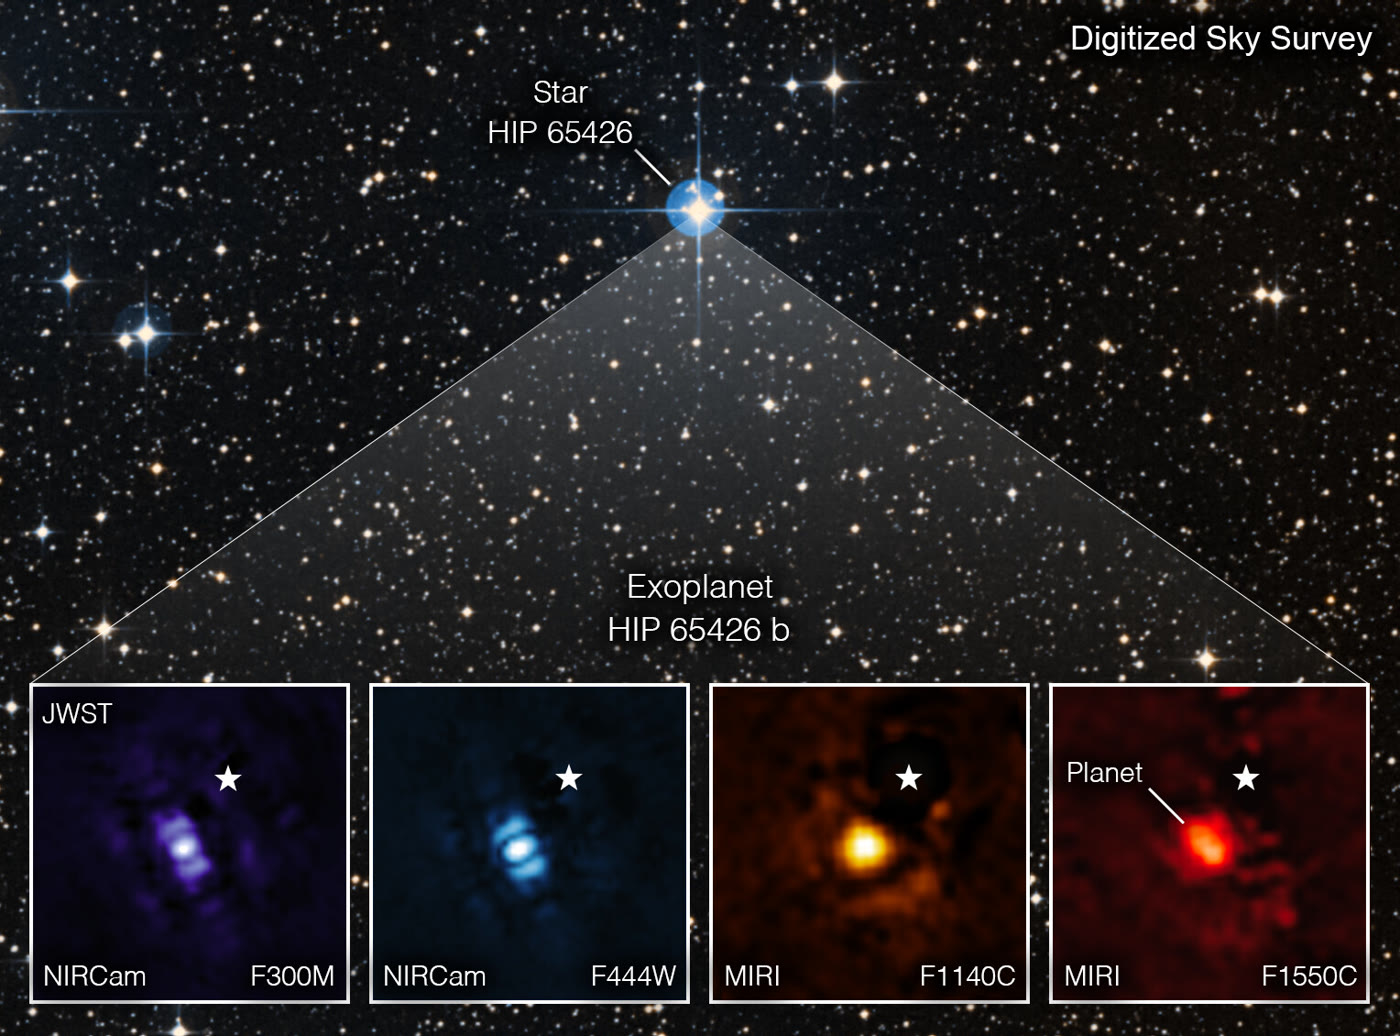
\includegraphics[width=0.86\linewidth]{images/book5/b3-hip65426b.jpg}
\par\smallskip{\small The first exoplanet imaged by the James Webb Space
Telescope, HIP~65426~b, in four infrared filters (bottom; top, the
star's field in a ground-based sky survey); the light of
the star, at the position of the star symbol, is blocked by the
\omterm{def:b3:exoplanets:imaging}{coronagraphs}. The planet is a young gas giant of about 6 to 8
Jupiter masses, some 15 to 20 million years old, about a hundred times
farther from its star than the Earth is from the Sun. Image NASA/ESA/CSA,
A~Carter (UCSC), the ERS~1386 team, and A.~Pagan (STScI), CC
BY~4.0.}\label{fig:b3:exoplanets:hip65426}
\end{omfigure}
% ledger: photo:b3-hip65426b

A fourth method uses gravity as a lens. When a star passes almost exactly
in front of a more distant one, its gravity bends the light of the
background star and brightens it for a few weeks; a planet of the lensing
star adds a short blip.

\begin{definition}[Gravitational microlensing; Einstein radius]\label{def:b3:exoplanets:microlensing}
\emph{Gravitational microlensing}\index{gravitational microlensing} is the
temporary brightening of a background star when a foreground star, the
lens, passes close to the line of sight; the images it forms are too close
together to be resolved. The \emph{Einstein radius}\index{Einstein radius}
is the angular radius $\theta_\mathrm E$ of the ring into which a point
lens of mass $M$ at the distance $D_L$ would turn a source at the
distance $D_S$ exactly behind it:
\[
\theta_\mathrm E = \sqrt{\frac{4GM}{c^2}\,\frac{D_S - D_L}{D_L D_S}} .
\]
\end{definition}

\begin{proposition}[Point-lens magnification]\label{prop:b3:exoplanets:magnification}
A source at the angular distance $u\,\theta_\mathrm E$ from a point lens
is brightened by the factor
\[
A(u) = \frac{u^2 + 2}{u\sqrt{u^2 + 4}} .
\]
\end{proposition}

\admitted

Both results come from the bending of light by a mass in general
relativity. For a lens of half a solar mass halfway to a source
\qty{8}{kpc} away, $\theta_\mathrm E = \qty{0.71}{mas}$, and the Einstein
ring, at the distance of the lens, has a radius of \qty{2.9}{au}. At
$u = 1$ the source is brightened 1.34 times, at $u = 0.1$ ten times. A
planet near the Einstein ring of its star adds a short deviation to the
light curve. Microlensing thus finds planets a few astronomical units
from their stars, cold planets that transits and radial velocities miss,
but each event happens once and is never repeated. In an event of 2003,
published the next year, a deviation lasting about seven days was
explained only by a companion of $\num{0.0039}$ times the mass of the
lens: a planet of about 1.5 Jupiter masses some \qty{3}{au} from its
star.
% ledger: const:G, const:c, sun:mass, iau:parsec, const:au, bond04:ogle235

\begin{omfigure}
\centering
\begin{tikzpicture}[scale=0.95]
\fill (0,0) circle (0.06) node[below=2pt, font=\scriptsize] {source};
\fill[omDef] (3.2,0) circle (0.09); \node[font=\scriptsize, omDef] at (3.2,-1.15) {lens};
\draw[omDef] (3.2,0) ellipse (0.12 and 0.9);
\fill (6.4,0) circle (0.06) node[below=2pt, font=\scriptsize] {observer};
\draw[thick, orange!80!black] (0,0) -- (3.2,0.9) -- (6.4,0);
\draw[thick, orange!80!black] (0,0) -- (3.2,-0.9) -- (6.4,0);
\draw[densely dashed, black!50] (6.4,0) -- (0,1.8) node[left, font=\scriptsize] {image};
\draw[densely dotted, black!50] (0,0) -- (6.4,0);
\draw[<->] (3.55,0) -- (3.55,0.9) node[midway, right, font=\scriptsize] {$R_\mathrm E$};
\draw[<->, black!60] (0,-1.5) -- (3.2,-1.5) node[midway, below, font=\scriptsize] {$D_S - D_L$};
\draw[<->, black!60] (3.2,-1.5) -- (6.4,-1.5) node[midway, below, font=\scriptsize] {$D_L$};
\end{tikzpicture}\hfill
\begin{tikzpicture}
\begin{axis}[width=0.48\linewidth, height=0.42\linewidth,
  xmin=-3, xmax=3, ymin=0.8, ymax=12, ymode=log,
  ytick={1,2,5,10}, yticklabels={1,2,5,10},
  xlabel={time ($t_\mathrm E$)}, ylabel={magnification $A$},
  tick label style={font=\scriptsize}, label style={font=\small},
  legend style={font=\scriptsize, at={(0.5,-0.30)}, anchor=north, legend columns=3, draw=none, cells={anchor=west}, /tikz/every even column/.append style={column sep=1em}}]
\addplot[thick, omDef] table[x=t_tE, y=A01] {figdata/out/bachelor-3-rv_transit-lens.dat};
\addlegendentry{$u_0 = 0.1$}
\addplot[thick, dashed, red!70!black] table[x=t_tE, y=A03] {figdata/out/bachelor-3-rv_transit-lens.dat};
\addlegendentry{$0.3$}
\addplot[thick, dotted, black] table[x=t_tE, y=A10] {figdata/out/bachelor-3-rv_transit-lens.dat};
\addlegendentry{$1$}
\end{axis}
\end{tikzpicture}
\par\smallskip{\small Left: the geometry of a gravitational lens, not to
scale; rays from the source pass the lens at about the \omterm{def:b3:exoplanets:microlensing}{Einstein radius}
$R_\mathrm E = \theta_\mathrm E D_L$ and reach the observer, who sees the
source displaced to the image. Right: the magnification of a point source
by a point lens against time, in units of the time $t_\mathrm E$ the lens
takes to move by one \omterm{def:b3:exoplanets:microlensing}{Einstein radius}, for three distances of closest
approach $u_0$ (in Einstein radii).}\label{fig:b3:exoplanets:microlensing}
\end{omfigure}

Every method has its own bias, and the catalogue of known planets
reflects them. Radial velocities favour massive planets close to their
stars; transits favour large planets close to their stars, and need the
orbit edge-on; microlensing finds planets of a few astronomical units;
imaging finds young giants tens or hundreds of astronomical units out.
The figure below shows the result: each method fills its own region, and
the Solar System's planets fall mostly in the gaps between them.

\begin{dated}{2026}
On 23 October 2026 the NASA Exoplanet Archive listed 6451 confirmed
planets. By method of discovery: 4785 by transits, 1204 by radial
velocity, 292 by microlensing, 98 by imaging, 29 by \omterm{def:b3:exoplanets:ttv}{transit-timing
variations} and the rest by rarer methods, among them the first ones of
all, found in 1992 around a pulsar by the timing of its pulses. The first
discoveries by radial velocity date from 1995, by transit from 2002, by
microlensing and imaging from 2004.
\end{dated}
% ledger: data:b5-pscomp

\begin{omfigure}
\centering
\begin{tikzpicture}
\begin{axis}[width=0.86\linewidth, height=0.56\linewidth,
  xmode=log, ymode=log, xmin=0.004, xmax=2000, ymin=0.02, ymax=1e5,
  legend image post style={scale=2.2},
  xlabel={semi-major axis (au)}, ylabel={mass or minimum mass ($M_\oplus$)},
  tick label style={font=\scriptsize}, label style={font=\small},
  legend style={font=\scriptsize, at={(0.5,-0.20)}, anchor=north, legend columns=4, draw=none, cells={anchor=west}, /tikz/every even column/.append style={column sep=1em}}]
\addplot[only marks, mark=*, mark size=0.6pt, omDef, opacity=0.6] table[x=a_au, y=mass] {figdata/out/bachelor-3-exoplanet_archive-ma-tr.dat};
\addlegendentry{transit}
\addplot[only marks, mark=*, mark size=0.6pt, red!70!black, opacity=0.6] table[x=a_au, y=mass] {figdata/out/bachelor-3-exoplanet_archive-ma-rv.dat};
\addlegendentry{radial velocity}
\addplot[only marks, mark=triangle*, mark size=1.2pt, green!45!black] table[x=a_au, y=mass] {figdata/out/bachelor-3-exoplanet_archive-ma-ml.dat};
\addlegendentry{microlensing}
\addplot[only marks, mark=diamond*, mark size=1.5pt, orange!85!black] table[x=a_au, y=mass] {figdata/out/bachelor-3-exoplanet_archive-ma-im.dat};
\addlegendentry{imaging}
\addplot[only marks, mark=square*, mark size=1.6pt, black, forget plot] table[x=a_au, y=mass] {figdata/out/bachelor-3-exoplanet_archive-solar.dat};
\node[font=\scriptsize, anchor=west, fill=white, inner sep=1pt] at (axis cs:1.15,1.0) {Earth};
\node[font=\scriptsize, anchor=east, fill=white, inner sep=1pt] at (axis cs:0.63,0.82) {Venus};
\node[font=\scriptsize, anchor=east, fill=white, inner sep=1pt] at (axis cs:0.34,0.055) {Mercury};
\node[font=\scriptsize, anchor=west, fill=white, inner sep=1pt] at (axis cs:1.75,0.107) {Mars};
\node[font=\scriptsize, anchor=west, fill=white, inner sep=1pt] at (axis cs:6.0,318) {Jupiter};
\node[font=\scriptsize, anchor=west, fill=white, inner sep=1pt] at (axis cs:11,95) {Saturn};
\node[font=\scriptsize, anchor=north, fill=white, inner sep=1pt] at (axis cs:25,11) {Uranus, Neptune};
\end{axis}
\end{tikzpicture}
\par\smallskip{\small Confirmed planets with a measured mass (or \omterm{def:b3:exoplanets:rv}{minimum
mass}) and semi-major axis, by method of discovery (NASA Exoplanet
Archive, 23 October 2026: 1691 by transit, 1151 by radial velocity, 286
by microlensing, 94 by imaging), with the Solar System's planets (black
squares). Masses predicted from a \omterm{def:b3:exoplanets:mass-radius}{mass--radius relation} are left out. This research
has made use of the NASA Exoplanet Archive, which is operated by the
California Institute of Technology, under contract with the National
Aeronautics and Space Administration under the Exoplanet Exploration
Program.}\label{fig:b3:exoplanets:methods}
\end{omfigure}
% ledger: data:b5-pscomp, planet:Mercury.mass, planet:Venus.mass, planet:Earth.mass, planet:Mars.mass, planet:Jupiter.mass, planet:Saturn.mass, planet:Uranus.mass, planet:Neptune.mass, planet:Mercury.dist, planet:Venus.dist, planet:Earth.dist, planet:Mars.dist, planet:Jupiter.dist, planet:Saturn.dist, planet:Uranus.dist, planet:Neptune.dist

\section{What has been found}\label{sec:b3:exoplanets:found}

The first surprise was the \omterm{def:b3:exoplanets:classes}{hot Jupiters}, giant planets on orbits of a
few days. 51~Pegasi~b cannot have formed so close to its star; it must
have formed farther out, perhaps at a few astronomical units, beyond the
snow line of its disc, and migrated inwards through its interaction with
the disc, as theory had predicted.
% ledger: nobel19:migration

\begin{definition}[Hot Jupiter; super-Earth; sub-Neptune]\label{def:b3:exoplanets:classes}
A \emph{hot Jupiter}\index{hot Jupiter} is a giant planet on a close orbit,
usually taken as a \omterm{def:b3:exoplanets:rv}{minimum mass} above 0.1 Jupiter masses and a period
shorter than ten days. A \emph{super-Earth}\index{super-Earth} is a planet
larger than the Earth but smaller than the \omterm{def:b3:exoplanets:radius-valley}{radius valley}, that is up to
about 1.5 to 2 Earth radii, and therefore probably rocky. A \emph{sub-Neptune}\index{sub-Neptune}
is a planet above the \omterm{def:b3:exoplanets:radius-valley}{radius valley} but smaller than Neptune, about 2 to
4 Earth radii, whose radius requires an envelope of light gases or
volatiles.
\end{definition}
% ledger: wright12:hj, fulton17:gap, planet:Neptune.diameter, planet:Earth.diameter

\begin{definition}[Occurrence rate]\label{def:b3:exoplanets:occurrence}
The \emph{occurrence rate}\index{occurrence rate} of a class of planets is
the mean number of such planets per star, or the fraction of stars that
host one, in a given range of size (or mass) and period, after the
counts of a survey are corrected for the planets it could not detect:
those whose orbits are not aligned for a transit, and those too small or
too far to be seen.
\end{definition}

\omterm{def:b3:exoplanets:classes}{Hot Jupiters}, prominent in the catalogue because they are the easiest to
find, are rare: a radial-velocity survey of nearby Sun-like stars found
them around \qty[separate-uncertainty=true]{1.2 \pm 0.38}{\percent} of the stars. Small planets are
common. Searching the light curves of \num{42000} stars watched by the
Kepler space telescope, one study found 603 planets, ten of them Earth-sized (1 to 2
Earth radii) and receiving between one and four times the Earth's
sunlight; corrected for the transit probability and for the planets the
search would miss, \qty[separate-uncertainty=true]{11 \pm 4}{\percent} of Sun-like stars host such a
planet.
% ledger: wright12:hj, petigura13:eta

The sizes of small planets are not spread evenly. Among close-in planets
measured precisely, those of 1.5 to 2.0 Earth radii are at least twice
rarer than those just smaller or just larger.

\begin{definition}[Radius valley]\label{def:b3:exoplanets:radius-valley}
The \emph{radius valley}\index{radius valley} is the deficit of planets
with radii between about 1.5 and 2.0 Earth radii among planets with
periods shorter than about a hundred days; it separates the \omterm{def:b3:exoplanets:classes}{super-Earths}
from the \omterm{def:b3:exoplanets:classes}{sub-Neptunes}.
\end{definition}
% ledger: fulton17:gap

The valley is read as the trace of escape. A rocky core born with a
hydrogen and helium envelope of only a few percent of its mass has twice
the radius of the bare core. Close to a young, active star, such an
envelope is heated and lost by \omterm{def:b3:planetary-atmospheres:hydrodynamic}{hydrodynamic escape}: by the star's
high-energy radiation during the first hundred million years
(photoevaporation), or by the heat of the cooling core itself (core-powered
mass loss). The models herd planets into bare cores of about 1.3 Earth
radii and planets of twice that size; few are left in between. The two
mechanisms depend differently on the star, and planets around stars of
different types may tell them apart.
% ledger: owen17:valley, ginzburg18:core-powered

\begin{omfigure}
\centering
\begin{tikzpicture}
\begin{axis}[name=pr, width=0.50\linewidth, height=0.50\linewidth,
  xmode=log, ymode=log, xmin=1, xmax=100, ymin=0.8, ymax=4,
  ytick={1,1.5,2,3,4}, yticklabels={1,1.5,2,3,4},
  xlabel={period (days)}, ylabel={radius ($R_\oplus$)},
  tick label style={font=\scriptsize}, label style={font=\small},
  title={(a)}, title style={font=\small}]
\fill[black!10] (axis cs:1,1.5) rectangle (axis cs:100,2.0);
\addplot[only marks, mark=*, mark size=0.5pt, omDef, opacity=0.7] table[x=period, y=radius] {figdata/out/bachelor-3-exoplanet_archive-pr.dat};
\end{axis}
\begin{axis}[at={(pr.east)}, anchor=west, xshift=0.09\linewidth,
  width=0.42\linewidth, height=0.50\linewidth,
  xmode=log, xmin=0.8, xmax=4, ymin=0, ymax=185,
  xtick={1,1.5,2,3,4}, xticklabels={1,1.5,2,3,4},
  xlabel={radius ($R_\oplus$)}, ylabel={number of planets},
  tick label style={font=\scriptsize}, label style={font=\small},
  title={(b)}, title style={font=\small}]
\fill[black!10] (axis cs:1.5,0) rectangle (axis cs:2.0,185);
\addplot[const plot mark left, thick, omDef, fill=omDef!25] table[x=r, y=n] {figdata/out/bachelor-3-exoplanet_archive-histstep.dat} \closedcycle;
\end{axis}
\end{tikzpicture}
\par\smallskip{\small (a)~Transiting planets with radii known to better
than \qty{10}{\percent}, around stars smaller than two solar radii, with
periods of 1 to 100 days (2370 planets, NASA Exoplanet Archive, 23
October 2026); shaded, the \omterm{def:b3:exoplanets:radius-valley}{radius valley} of 1.5 to 2.0 Earth radii.
(b)~The same planets counted in 20 bins of equal width in $\log R$.
The counts are not corrected for the planets the surveys miss, which are
more numerous among the small ones; the valley shows nonetheless.}\label{fig:b3:exoplanets:valley}
\end{omfigure}
% ledger: data:b5-pscomp, fulton17:gap

\begin{definition}[Mass--radius relation]\label{def:b3:exoplanets:mass-radius}
The \emph{mass--radius relation}\index{mass--radius relation} of a
composition is the radius of a planet of that composition as a function
of its mass, computed from the equations of state of its materials in
hydrostatic equilibrium; a measured planet is compared with the
relations of candidate compositions.
\end{definition}

A rocky planet is compressed by its own weight, and its radius grows
more slowly than $M^{1/3}$. A fit to models of two-layer planets built on
the Earth's seismic model gives $R/R_\oplus = (1.07 - 0.21\,C)
(M/M_\oplus)^{1/3.7}$, for 1 to 8 Earth masses and a core mass fraction
$C$ from 0 to 0.4; fitted to the Earth, Venus and a few small
exoplanets, it gives $C = 0.26 \pm 0.07$. An
iron planet is smaller at the same mass; a planet half water, larger;
an envelope of hydrogen of only two percent of the mass makes a planet of
five Earth masses \num{2.6} Earth radii across, the size of a
\omterm{def:b3:exoplanets:classes}{sub-Neptune}. The degeneracy is real: a radius and a mass give one
density, and several mixtures of iron, rock, water and gas can share it.
The rocky planet Kepler-10~b, at 3.24 Earth masses and 1.47 Earth radii,
has a mean density of \qty{5.6}{g.cm^{-3}}; the gas giant WASP-39~b,
at 89 Earth masses and 14.3 Earth radii, \qty{0.17}{g.cm^{-3}}.
% ledger: zeng16:rocky, data:b5-zeng, data:b5-pscomp

\begin{omfigure}
\centering
\begin{tikzpicture}
\begin{axis}[width=0.86\linewidth, height=0.58\linewidth,
  xmode=log, ymode=log, xmin=0.3, xmax=5000, ymin=0.5, ymax=25,
  ytick={0.5,1,2,4,10,20}, yticklabels={0.5,1,2,4,10,20},
  xlabel={mass ($M_\oplus$)}, ylabel={radius ($R_\oplus$)},
  tick label style={font=\scriptsize}, label style={font=\small},
  legend style={font=\scriptsize, at={(0.5,-0.20)}, anchor=north, legend columns=3, draw=none, cells={anchor=west}, /tikz/every even column/.append style={column sep=1em}}]
\addplot[only marks, mark=*, mark size=0.6pt, black!35, forget plot] table[x=mass, y=radius] {figdata/out/bachelor-3-exoplanet_archive-mr.dat};
\addplot[thick, black] table[x=mass, y=radius] {figdata/out/bachelor-3-exoplanet_archive-zeng-iron.dat};
\addlegendentry{pure iron}
\addplot[thick, brown!70!black] table[x=mass, y=radius] {figdata/out/bachelor-3-exoplanet_archive-zeng-earthlike.dat};
\addlegendentry{Earth-like rock}
\addplot[thick, omDef] table[x=mass, y=radius] {figdata/out/bachelor-3-exoplanet_archive-zeng-water50.dat};
\addlegendentry{50\,\% water}
\addplot[thick, dashed, orange!85!black] table[x=mass, y=radius] {figdata/out/bachelor-3-exoplanet_archive-zeng-h2-2pc.dat};
\addlegendentry{rock + 2\,\% hydrogen}
\addplot[only marks, mark=square*, mark size=1.8pt, red!70!black] table[x=mass, y=radius] {figdata/out/bachelor-3-exoplanet_archive-solar.dat};
\addlegendentry{Solar System}
\node[font=\scriptsize, anchor=north west] at (axis cs:1.05,0.97) {Earth};
\node[font=\scriptsize, anchor=south east] at (axis cs:0.80,0.97) {Venus};
\node[font=\scriptsize, anchor=south east, fill=white, inner sep=1pt] at (axis cs:13.5,4.3) {Uranus, Neptune};
\node[font=\scriptsize, anchor=east, fill=white, inner sep=1pt] at (axis cs:80,9.45) {Saturn};
\node[font=\scriptsize, anchor=north, fill=white, inner sep=1pt] at (axis cs:318,10.3) {Jupiter};
\end{axis}
\end{tikzpicture}
\par\smallskip{\small Mass and radius of 1078 transiting planets whose
mass is measured to better than \qty{25}{\percent} and radius to better
than \qty{10}{\percent} (grey; NASA Exoplanet Archive, 23 October 2026),
with model curves of L.~Zeng and others (2016, 2019): pure iron;
Earth-like rock, a third iron and two thirds silicate; half water on such
a core, at \qty{500}{K}; an Earth-like core with a hydrogen envelope of
\qty{2}{\percent} of its mass, at \qty{500}{K}. Red squares: the Solar
System's planets (Mercury and Mars lie off the scale, to the
left).}\label{fig:b3:exoplanets:mass-radius}
\end{omfigure}
% ledger: data:b5-pscomp, data:b5-zeng, planet:Earth.mass, planet:Earth.diameter, planet:Venus.mass, planet:Venus.diameter, planet:Jupiter.mass, planet:Jupiter.diameter, planet:Saturn.mass, planet:Saturn.diameter, planet:Uranus.mass, planet:Uranus.diameter, planet:Neptune.mass, planet:Neptune.diameter

\section{Atmospheres}\label{sec:b3:exoplanets:atmospheres}

A transiting planet can be weighed and measured; it can also be smelled.
During a transit, a thin ring of the planet's atmosphere stands against
the star, and starlight filters through it. At wavelengths where a gas
of the atmosphere absorbs, the ring is opaque higher up, and the planet
looks larger.

\begin{definition}[Transmission spectroscopy; secondary eclipse]\label{def:b3:exoplanets:transmission}
\emph{Transmission spectroscopy}\index{transmission spectroscopy} measures
the \omterm{def:b3:exoplanets:transit}{transit depth} as a function of wavelength, to detect the gases of the
atmosphere that the starlight crosses at the planet's limb. A
\emph{secondary eclipse}\index{secondary eclipse} is the passage of a
planet behind its star, half an orbit after the transit on a circular
orbit; the drop of the system's flux then measures the light of the
planet's day side.
\end{definition}

\begin{proposition}[Transmission signal]\label{prop:b3:exoplanets:transmission}
An atmosphere of scale height $H \ll R_p$, made opaque over $n$ more
scale heights at the wavelength of an absorption band than at
neighbouring wavelengths, deepens the transit there by
\[
\Delta\delta \approx n\,\frac{2HR_p}{R_\star^2} .
\]
\end{proposition}

\begin{proof}
The planet's apparent radius grows from $R_p$ to $R_p + nH$, so the
depth $(R_p + nH)^2/R_\star^2$ grows by $(2nHR_p + n^2H^2)/R_\star^2$,
which is $2nHR_p/R_\star^2$ when $nH \ll R_p$.
\end{proof}

The scale height $H = kT/\bar m g$ is large for a hot planet of low
gravity with light hydrogen air, small for a cool, dense planet with
heavy air. For the Earth seen against the Sun, with $H = \qty{8}{km}$,
each scale height adds 0.2 parts per million; for a hot, puffy gas giant,
several hundred.
% ledger: planet:Earth.diameter, sun:R

\begin{proposition}[Secondary-eclipse depth]\label{prop:b3:exoplanets:eclipse}
If the day side of a planet radiates as a black body at the temperature
$T_d$ and the star as one at $T_\star$, the \omterm{def:b3:exoplanets:transmission}{secondary eclipse} at the
wavelength $\lambda$ has the depth
\[
\delta_\mathrm{ecl} \approx \left(\frac{R_p}{R_\star}\right)^2
  \frac{B_\lambda(T_d)}{B_\lambda(T_\star)},
\]
with $B_\lambda$ Planck's law, the planet's reflected light neglected.
\end{proposition}

\begin{proof}
Just before the eclipse the observer receives the star's light, in
proportion to $\pi R_\star^2 B_\lambda(T_\star)$, plus the day side's,
in proportion to $\pi R_p^2 B_\lambda(T_d)$; during the eclipse only the
star's. The fractional drop is the ratio of the planet's term to the
star's, the planet's being small.
\end{proof}

The eclipse is deepest in the infrared, where the cool planet is
brightest relative to its star: it gives the day side's temperature, and
a hot day side next to a cool night side reveals a thin or absent
atmosphere that does not carry heat around.

\begin{dated}{2023}
In 2022 the transmission spectrum of the gas giant WASP-39~b, measured
between 3.0 and \qty{5.5}{\micro m} by the James Webb Space Telescope,
showed a prominent absorption band of carbon dioxide at
\qty{4.3}{\micro m}, at 26 standard deviations, where earlier photometry
had only hinted at the gas: its first clear identification in an
exoplanet's atmosphere. In 2023 five \omterm{def:b3:exoplanets:transmission}{secondary eclipses} of the
Earth-sized TRAPPIST-1~b, which receives four times the Earth's sunlight
from a cool, small star, were measured at \qty{15}{\micro m}. They fit
heat re-radiated from the day side alone, with no detectable carbon
dioxide: the planet has little or no atmosphere to carry heat to its
night side.
\end{dated}
% ledger: jwst23:wasp39-co2, greene23:trappist1b

The rocky planets of the habitable zones of small stars are within reach
of these methods, at the limit. Whether they kept their air against the
escape processes of the previous chapter is now an observational
question.

\section{Exercises}

\begin{exercise}[$\star$]\label{exo:b3:exoplanets:1}
(a)~Compute the radial-velocity semi-amplitude of the Sun caused by
Jupiter (mass \qty{1898e24}{kg}, period \num{4331}~days, eccentricity
0.049) and by the Earth (mass \qty{5.97e24}{kg}, period \num{365.2}~days,
eccentricity 0.017). The Sun's mass is \qty{1.9884e30}{kg}.
(b)~Convert the precisions \qty{3.5}{km/h} and \qty{0.35}{km/h} into
metres per second, and compare.
\end{exercise}

\begin{exercise}[$\star$]\label{exo:b3:exoplanets:2}
(a)~Compute the \omterm{def:b3:exoplanets:transit}{transit depths} of Jupiter (radius \qty{71492}{km}) and of
the Earth (radius \qty{6378}{km}) across the Sun (radius
\qty{695700}{km}). (b)~Compute the probability that a randomly placed
observer sees each of them transit, with orbital radii of \qty{778.5}{}
and \qty{149.6}{\mega km}.
\end{exercise}

\begin{exercise}[$\star$]\label{exo:b3:exoplanets:3}
51~Pegasi~b gives its star a radial-velocity semi-amplitude of
\qty{59}{m.s^{-1}}, with a period of \qty{4.23}{d}. Taking the star's
mass equal to the Sun's, compute the planet's \omterm{def:b3:exoplanets:rv}{minimum mass}, in Jupiter
masses and in Earth masses, and the radius of its orbit.
\end{exercise}

\begin{exercise}[$\star$]\label{exo:b3:exoplanets:4}
A star of half a solar mass at \qty{4}{kpc} lenses a star at
\qty{8}{kpc} ($\qty{1}{pc} = \qty{3.0857e16}{m}$). (a)~Compute its
\omterm{def:b3:exoplanets:microlensing}{Einstein radius} in milliarcseconds and the radius of the Einstein ring,
in astronomical units, at the distance of the lens. (b)~Compute the
magnification at $u = 1$, $0.5$ and $0.1$. (c)~How long does the lens take
to cross one \omterm{def:b3:exoplanets:microlensing}{Einstein radius} if it moves across the line of sight at
\qty{200}{km.s^{-1}}?
\end{exercise}

\begin{exercise}[$\star\star$]\label{exo:b3:exoplanets:5}
A planet of radius ratio $p = 0.12$ orbits a star of one solar mass and
one solar radius in \qty{3.0}{d}. (a)~Compute $a/R_\star$. (b)~Compute
$T_{14}$ and $T_{23}$ for $b = 0$ and for $b = 0.7$, and the inclination
in the second case. (c)~How does the shape of the light curve tell a
central transit from a grazing one?
\end{exercise}

\begin{exercise}[$\star\star$]\label{exo:b3:exoplanets:6}
From the masses and radii of the Exoplanet Archive, compute the mean
densities of TRAPPIST-1~b (1.374 Earth masses, 1.116 Earth radii),
Kepler-10~b (3.24, 1.47), WASP-39~b (89.31, 14.34) and HD~209458~b (232.0,
15.58), with $M_\oplus = \qty{5.97e24}{kg}$ and $R_\oplus =
\qty{6378}{km}$. Which are rocky, which gaseous?
\end{exercise}

\begin{exercise}[$\star\star$]\label{exo:b3:exoplanets:7}
The radial velocity of a star with one planet on an eccentric orbit
ranges from $+\qty{50.4}{m.s^{-1}}$ to $-\qty{9.6}{m.s^{-1}}$, and the
velocity of the system's centre of mass is \qty{12.4}{m.s^{-1}}. Using the
eccentric form of the theorem, compute $K$ and $e\cos\omega$. Why can the
mean of the two extremes differ from $\gamma$?
\end{exercise}

\begin{exercise}[$\star\star$]\label{exo:b3:exoplanets:8}
WASP-39~b has 89.31 Earth masses and 14.34 Earth radii; its star 0.939
solar radii. Take a temperature of \qty{1100}{K} and a mean molecular
mass of \qty{2.3}{u} for its atmosphere. (a)~Compute its gravity, its
scale height and its \omterm{def:b3:exoplanets:transit}{transit depth}. (b)~Compute the transmission signal of
one scale height, and of an absorption band two scale heights high, in
parts per million.
\end{exercise}

\begin{exercise}[$\star\star$]\label{exo:b3:exoplanets:9}
TRAPPIST-1~b has a radius of 1.116 Earth radii; its star, 0.1192 solar
radii and \qty{2566}{K}. Compute the depth of its \omterm{def:b3:exoplanets:transmission}{secondary eclipse} at
\qty{15}{\micro m} for a day side at \qty{400}{K} and at \qty{500}{K}
($hc/k = \qty{0.014388}{m.K}$). Why is a measurement of the depth a
thermometer?
\end{exercise}

\begin{exercise}[$\star\star\star$]\label{exo:b3:exoplanets:10}
An invented red dwarf has 0.2 solar masses, 0.2 solar radii and a
luminosity of \num{0.005} solar luminosities. (a)~At what distance does a
planet receive the Earth's stellar flux, and what is its period?
(b)~Compute the semi-amplitude caused by a planet of one Earth mass
there, and compare it with the Earth's effect on the Sun. (c)~Compute the
\omterm{def:b3:exoplanets:transit}{transit depth} of an Earth-sized planet. Why are such stars favoured
targets in the search for rocky planets in habitable zones?
\end{exercise}

\begin{exercise}[$\star\star\star$]\label{exo:b3:exoplanets:11}
For the quadratic limb-darkening law, show that the mean intensity of
the disc is $I(1)(1 - u_1/3 - u_2/6)$. Deduce the depth, in units of
$p^2$, of a small planet at $r = 0$, $0.5$ and $0.9$ for $u_1 = 0.40$,
$u_2 = 0.25$. What error would a uniform-disc model make on the radius of
a planet observed at mid-transit with $b = 0$?
\end{exercise}

\begin{exercise}[$\star\star\star$]\label{exo:b3:exoplanets:12}
A survey watched \num{42000} Sun-like stars and searched them for
Earth-sized planets receiving one to four times the Earth's sunlight,
that is on orbits of 0.5 to \qty{1}{au}. (a)~Compute the transit
probability at 0.5, 0.7 and \qty{1}{au}. (b)~If \qty{11}{\percent} of the
stars host one such planet, at about \qty{0.7}{au}, how many transit?
(c)~The survey found ten. What does the difference measure, and why must
the \omterm{def:b3:exoplanets:occurrence}{occurrence rate} be corrected for it?
\end{exercise}

\section{Problem: A Planet Around Selene's Lamp}

\begin{problem}[{Weekend problem --- weighing, sizing and sniffing an
invented planet}]
\label{pb:b3:exoplanets:1}
Selene's Lamp is an invented K~dwarf of mass 0.80 solar masses, radius
0.76 solar radii and effective temperature \qty{5000}{K}. A
radial-velocity survey finds that its velocity varies sinusoidally with
a period of \qty{12.0}{d} and a semi-amplitude of \qty{2.59}{m.s^{-1}}. A
space telescope then sees transits of the same period, of depth
\num{838} parts per million and total duration $T_{14} = \qty{3.23}{h}$.
Take $M_\odot = \qty{1.9884e30}{kg}$, $R_\odot = \qty{695700}{km}$,
$L_\odot = \qty{3.828e26}{W}$, $M_\oplus = \qty{5.97e24}{kg}$,
$R_\oplus = \qty{6378}{km}$.

\medskip\noindent\textbf{Part I --- The radial velocity.}
\begin{enumerate}
\item Compute the radius of the orbit, in metres and in astronomical
  units, neglecting the planet's mass against the star's.
\item Compute the planet's orbital speed.
\item Compute the \omterm{def:b3:exoplanets:rv}{minimum mass} of the planet, in Earth masses.
\item Compute the radius of the star's own orbit about the centre of
  mass, and check that it gives the observed semi-amplitude.
\item By how many times does the signal exceed a precision of
  \qty{1}{m.s^{-1}}, and of \qty{0.1}{m.s^{-1}}?
\item If the orbit had $e = 0.2$ with the same $K$, by how much would the
  \omterm{def:b3:exoplanets:rv}{minimum mass} change?
\end{enumerate}

\medskip\noindent\textbf{Part II --- The transit.}
\begin{enumerate}[resume]
\item Compute the radius ratio $p = R_p/R_\star$.
\item Compute the radius of the planet, in kilometres and in Earth radii.
\item Compute $a/R_\star$.
\item Compute the duration of a central transit ($b = 0$).
\item From the observed $T_{14}$, compute the \omterm{def:b3:exoplanets:transit}{impact parameter}.
\item Compute the inclination of the orbit.
\item What was the probability that this planet transits, seen from a
  random direction?
\end{enumerate}

\medskip\noindent\textbf{Part III --- What is it made of?}
\begin{enumerate}[resume]
\item Compute the true mass of the planet.
\item Compute its mean density.
\item On the Earth-like rocky model curve, a planet of this mass would
  have a radius of 1.74 Earth radii. Compare, and say what the planet
  must contain besides rock.
\item Where does the planet lie with respect to the \omterm{def:b3:exoplanets:radius-valley}{radius valley}? Is it
  a \omterm{def:b3:exoplanets:classes}{super-Earth} or a \omterm{def:b3:exoplanets:classes}{sub-Neptune}?
\item Compute its surface gravity.
\end{enumerate}

\medskip\noindent\textbf{Part IV --- Its atmosphere.}
\begin{enumerate}[resume]
\item Compute the luminosity of the star, in watts and in solar
  luminosities.
\item Compute the stellar flux the planet receives, relative to the
  Earth's. Is it in the habitable zone?
\item With a Bond albedo of 0.3, compute its equilibrium temperature.
\item Compute the scale height of an atmosphere of hydrogen and helium
  (mean molecular mass \qty{2.3}{u}) at that temperature.
\item Compute the transmission signal of one scale height, and of a
  water band two scale heights high, in parts per million.
\item Compute the same for an atmosphere of steam (\qty{18}{u}). Which of
  the two could a space telescope with a precision of about ten parts per
  million tell apart from a flat spectrum?
\item Give the planet's mean density, in grams per cubic centimetre, to
  two significant figures.
\end{enumerate}
\end{problem}
% ledger: sun:mass, sun:R, sun:L, planet:Earth.mass, planet:Earth.diameter, const:G, const:kB, const:sigma, nist:u, data:b5-zeng, fulton17:gap, eso:espresso
